\documentclass[tikz,border=8pt]{standalone}
\usepackage{amsmath}
\usetikzlibrary{arrows.meta,positioning}
\begin{document}
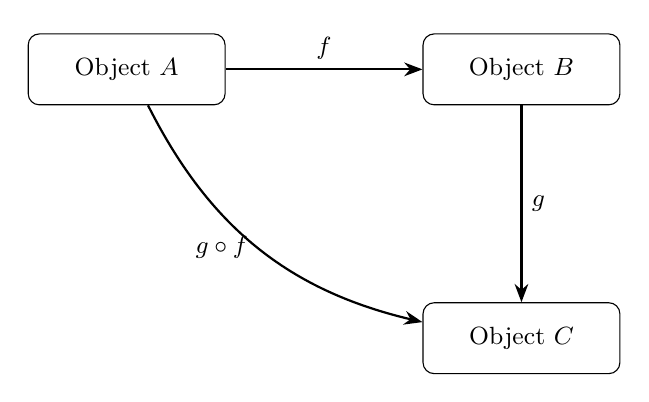
\begin{tikzpicture}[
  node distance=2.5cm,
  every node/.style={font=\small},
  box/.style={
    draw,
    rounded corners,
    minimum width=2.5cm,
    minimum height=0.9cm,
    align=center
  },
  arrow/.style={->, >=Stealth, thick}
]
\node[box] (A) {Object $A$};
\node[box, right=of A] (B) {Object $B$};
\node[box, below=of B] (C) {Object $C$};
\draw[arrow] (A) -- node[above] {$f$} (B);
\draw[arrow] (B) -- node[right] {$g$} (C);
\draw[arrow] (A) to[bend right=25] node[left] {$g \circ f$} (C);
\end{tikzpicture}
\end{document}
